% Figures for NeuroMCP-Agent Paper
% This file contains TikZ/PGF code for generating publication-quality figures

\documentclass[tikz,border=10pt]{standalone}
\usepackage{tikz}
\usepackage{pgfplots}
\usepackage{pgfplotstable}
\pgfplotsset{compat=1.18}
\usetikzlibrary{shapes,arrows,positioning,fit,backgrounds,calc,decorations.pathreplacing}

\begin{document}

%% ============================================
%% FIGURE 1: System Architecture
%% ============================================
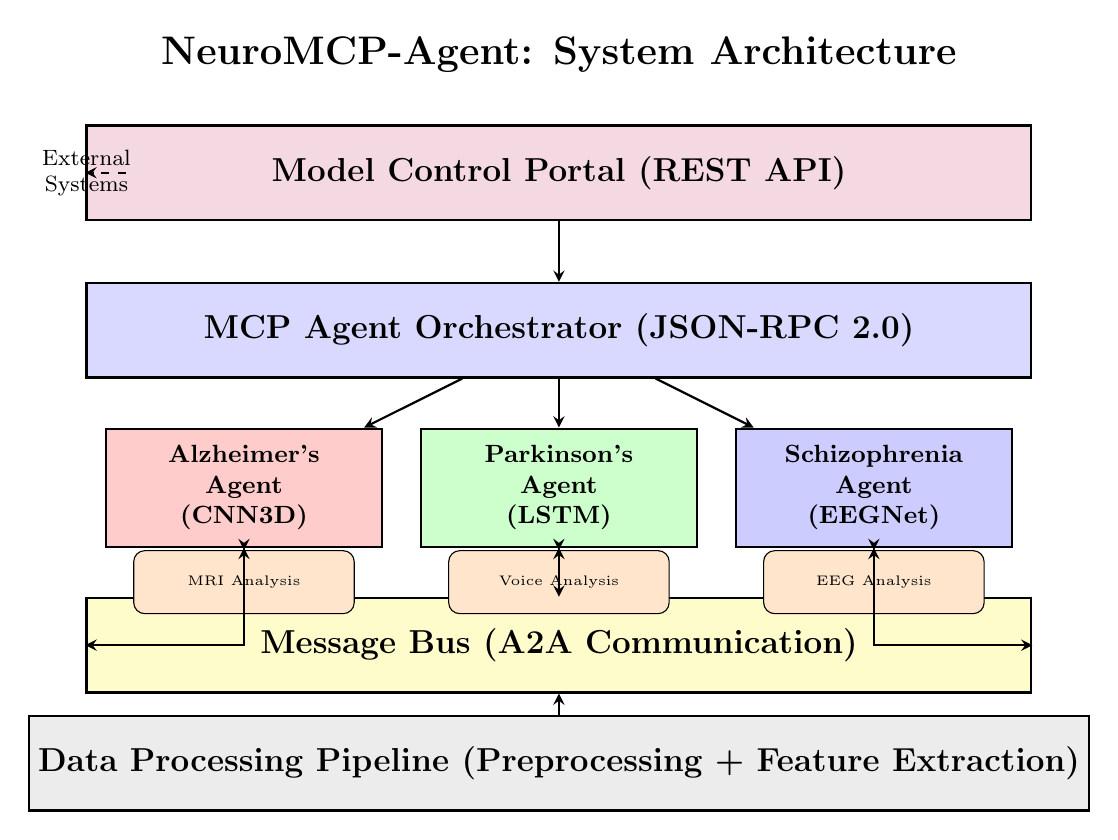
\begin{tikzpicture}[
    node distance=1.5cm,
    layer/.style={rectangle, draw=black, thick, minimum width=12cm, minimum height=1.2cm, fill=blue!10, font=\large\bfseries},
    agent/.style={rectangle, draw=black, thick, minimum width=3.5cm, minimum height=1.5cm, fill=green!20, font=\small\bfseries, align=center},
    tool/.style={rectangle, draw=black, rounded corners, minimum width=2.8cm, minimum height=0.8cm, fill=orange!20, font=\tiny},
    arrow/.style={->, thick, >=stealth},
    doublearrow/.style={<->, thick, >=stealth}
]

% Title
\node[font=\Large\bfseries] at (0,8.5) {NeuroMCP-Agent: System Architecture};

% Layer 1: Model Control Portal
\node[layer, fill=purple!15] (portal) at (0,7) {Model Control Portal (REST API)};

% Layer 2: MCP Orchestrator
\node[layer, fill=blue!15] (mcp) at (0,5) {MCP Agent Orchestrator (JSON-RPC 2.0)};

% Layer 3: Disease Agents
\node[agent, fill=red!20] (alz) at (-4,3) {Alzheimer's\\Agent\\(CNN3D)};
\node[agent, fill=green!20] (park) at (0,3) {Parkinson's\\Agent\\(LSTM)};
\node[agent, fill=blue!20] (schiz) at (4,3) {Schizophrenia\\Agent\\(EEGNet)};

% Layer 4: Message Bus
\node[layer, fill=yellow!20] (bus) at (0,1) {Message Bus (A2A Communication)};

% Layer 5: Data Processing
\node[layer, fill=gray!15] (data) at (0,-0.5) {Data Processing Pipeline (Preprocessing + Feature Extraction)};

% Tools for each agent
\node[tool] (t1) at (-4,1.8) {MRI Analysis};
\node[tool] (t2) at (0,1.8) {Voice Analysis};
\node[tool] (t3) at (4,1.8) {EEG Analysis};

% Arrows
\draw[arrow] (portal) -- (mcp);
\draw[arrow] (mcp) -- (alz);
\draw[arrow] (mcp) -- (park);
\draw[arrow] (mcp) -- (schiz);
\draw[arrow] (alz) -- (t1);
\draw[arrow] (park) -- (t2);
\draw[arrow] (schiz) -- (t3);
\draw[doublearrow] (bus) -- ++(-4,0) -- (alz);
\draw[doublearrow] (bus) -- (park);
\draw[doublearrow] (bus) -- ++(4,0) -- (schiz);
\draw[arrow] (data) -- (bus);

% External labels
\node[font=\footnotesize, align=center] at (-6,7) {External\\Systems};
\draw[arrow, dashed] (-5.5,7) -- (portal);

\end{tikzpicture}

%% ============================================
%% FIGURE 2: MCP Protocol Flow
%% ============================================
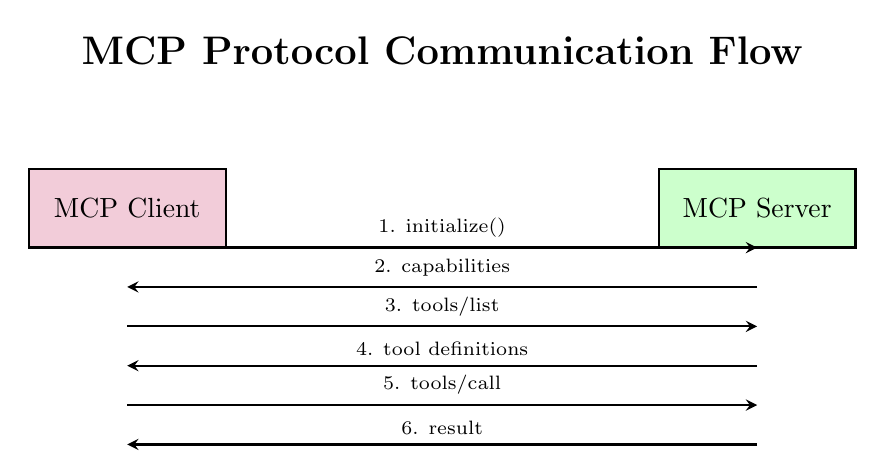
\begin{tikzpicture}[
    node distance=2cm,
    block/.style={rectangle, draw, thick, minimum width=2.5cm, minimum height=1cm, fill=blue!10},
    arrow/.style={->, thick, >=stealth}
]

\node[font=\Large\bfseries] at (0,5) {MCP Protocol Communication Flow};

% Components
\node[block, fill=purple!20] (client) at (-4,3) {MCP Client};
\node[block, fill=green!20] (server) at (4,3) {MCP Server};

% Messages
\draw[arrow] (-4,2.5) -- node[above, font=\scriptsize] {1. initialize()} (4,2.5);
\draw[arrow] (4,2) -- node[above, font=\scriptsize] {2. capabilities} (-4,2);
\draw[arrow] (-4,1.5) -- node[above, font=\scriptsize] {3. tools/list} (4,1.5);
\draw[arrow] (4,1) -- node[above, font=\scriptsize] {4. tool definitions} (-4,1);
\draw[arrow] (-4,0.5) -- node[above, font=\scriptsize] {5. tools/call} (4,0.5);
\draw[arrow] (4,0) -- node[above, font=\scriptsize] {6. result} (-4,0);

\end{tikzpicture}

%% ============================================
%% FIGURE 3: Performance Comparison Bar Chart
%% ============================================
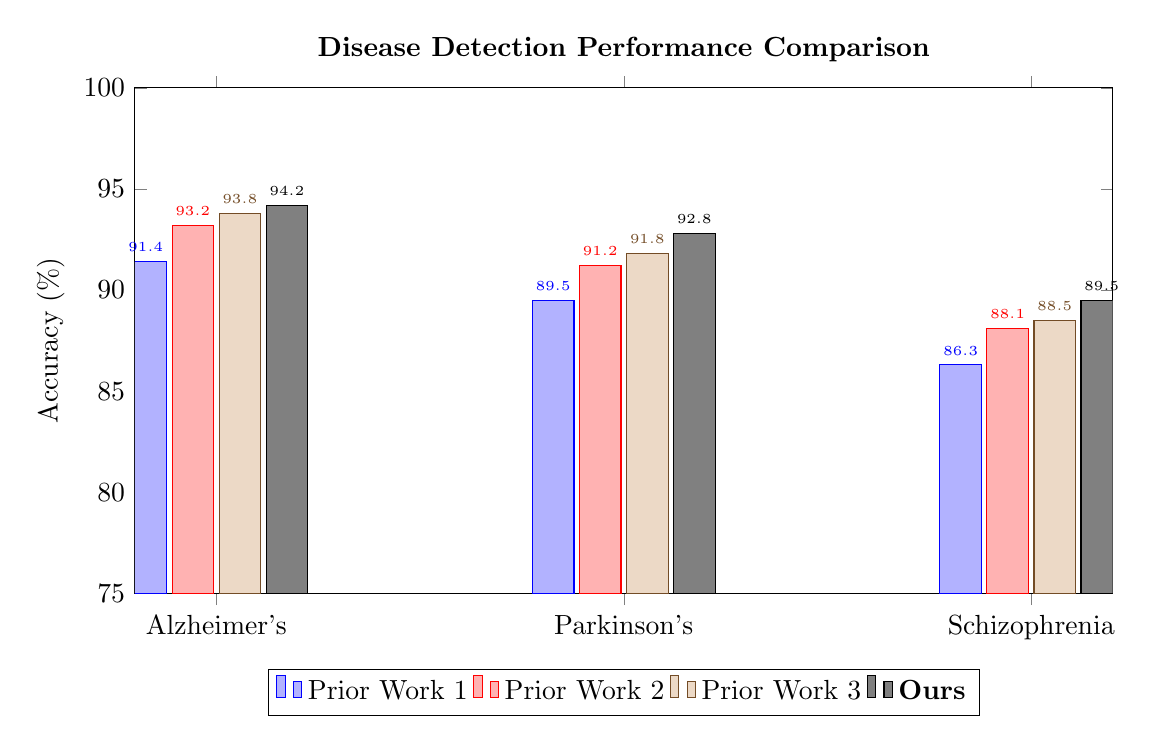
\begin{tikzpicture}
\begin{axis}[
    title={\textbf{Disease Detection Performance Comparison}},
    ybar,
    bar width=15pt,
    width=14cm,
    height=8cm,
    ylabel={Accuracy (\%)},
    symbolic x coords={Alzheimer's, Parkinson's, Schizophrenia},
    xtick=data,
    ymin=75,
    ymax=100,
    legend style={at={(0.5,-0.15)}, anchor=north, legend columns=4},
    nodes near coords,
    nodes near coords align={vertical},
    every node near coord/.append style={font=\tiny},
]
\addplot coordinates {(Alzheimer's,91.4) (Parkinson's,89.5) (Schizophrenia,86.3)};
\addplot coordinates {(Alzheimer's,93.2) (Parkinson's,91.2) (Schizophrenia,88.1)};
\addplot coordinates {(Alzheimer's,93.8) (Parkinson's,91.8) (Schizophrenia,88.5)};
\addplot coordinates {(Alzheimer's,94.2) (Parkinson's,92.8) (Schizophrenia,89.5)};
\legend{Prior Work 1, Prior Work 2, Prior Work 3, \textbf{Ours}}
\end{axis}
\end{tikzpicture}

%% ============================================
%% FIGURE 4: ROC Curves
%% ============================================
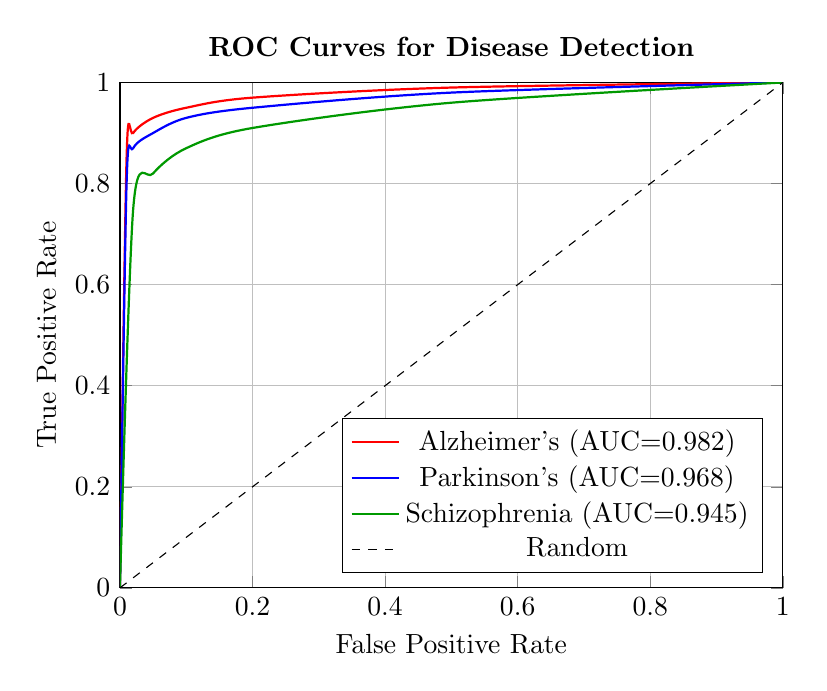
\begin{tikzpicture}
\begin{axis}[
    title={\textbf{ROC Curves for Disease Detection}},
    xlabel={False Positive Rate},
    ylabel={True Positive Rate},
    xmin=0, xmax=1,
    ymin=0, ymax=1,
    width=10cm,
    height=8cm,
    legend pos=south east,
    grid=major,
]
% Alzheimer's ROC
\addplot[red, thick, smooth] coordinates {
    (0,0) (0.01,0.85) (0.02,0.90) (0.05,0.93) (0.1,0.95) (0.2,0.97) (0.5,0.99) (1,1)
};
% Parkinson's ROC
\addplot[blue, thick, smooth] coordinates {
    (0,0) (0.01,0.80) (0.02,0.87) (0.05,0.90) (0.1,0.93) (0.2,0.95) (0.5,0.98) (1,1)
};
% Schizophrenia ROC
\addplot[green!60!black, thick, smooth] coordinates {
    (0,0) (0.02,0.75) (0.05,0.82) (0.1,0.87) (0.2,0.91) (0.5,0.96) (1,1)
};
% Diagonal
\addplot[black, dashed] coordinates {(0,0) (1,1)};

\legend{Alzheimer's (AUC=0.982), Parkinson's (AUC=0.968), Schizophrenia (AUC=0.945), Random}
\end{axis}
\end{tikzpicture}

%% ============================================
%% FIGURE 5: Confusion Matrix - Alzheimer's
%% ============================================
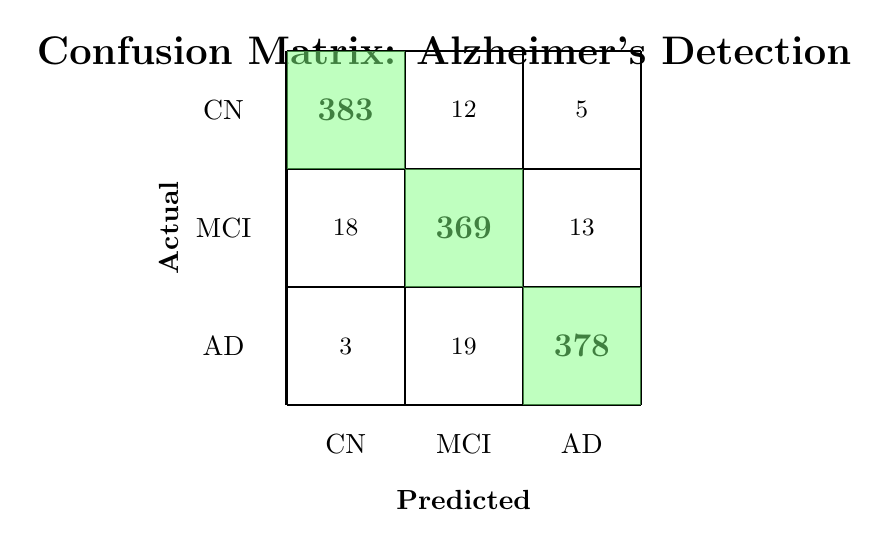
\begin{tikzpicture}
\node[font=\Large\bfseries] at (2,4.5) {Confusion Matrix: Alzheimer's Detection};

\draw[step=1.5cm,black,thick] (0,0) grid (4.5,4.5);

% Labels
\node at (-0.8,3.75) {CN};
\node at (-0.8,2.25) {MCI};
\node at (-0.8,0.75) {AD};
\node at (0.75,-0.5) {CN};
\node at (2.25,-0.5) {MCI};
\node at (3.75,-0.5) {AD};

\node[rotate=90] at (-1.5,2.25) {\textbf{Actual}};
\node at (2.25,-1.2) {\textbf{Predicted}};

% Values (normalized)
\node[font=\large] at (0.75,3.75) {\textbf{383}};
\node[font=\small] at (2.25,3.75) {12};
\node[font=\small] at (3.75,3.75) {5};

\node[font=\small] at (0.75,2.25) {18};
\node[font=\large] at (2.25,2.25) {\textbf{369}};
\node[font=\small] at (3.75,2.25) {13};

\node[font=\small] at (0.75,0.75) {3};
\node[font=\small] at (2.25,0.75) {19};
\node[font=\large] at (3.75,0.75) {\textbf{378}};

% Color coding (diagonal = green, off-diagonal = red intensity)
\fill[green!50, opacity=0.5] (0,3) rectangle (1.5,4.5);
\fill[green!50, opacity=0.5] (1.5,1.5) rectangle (3,3);
\fill[green!50, opacity=0.5] (3,0) rectangle (4.5,1.5);

\end{tikzpicture}

%% ============================================
%% FIGURE 6: Feature Importance
%% ============================================
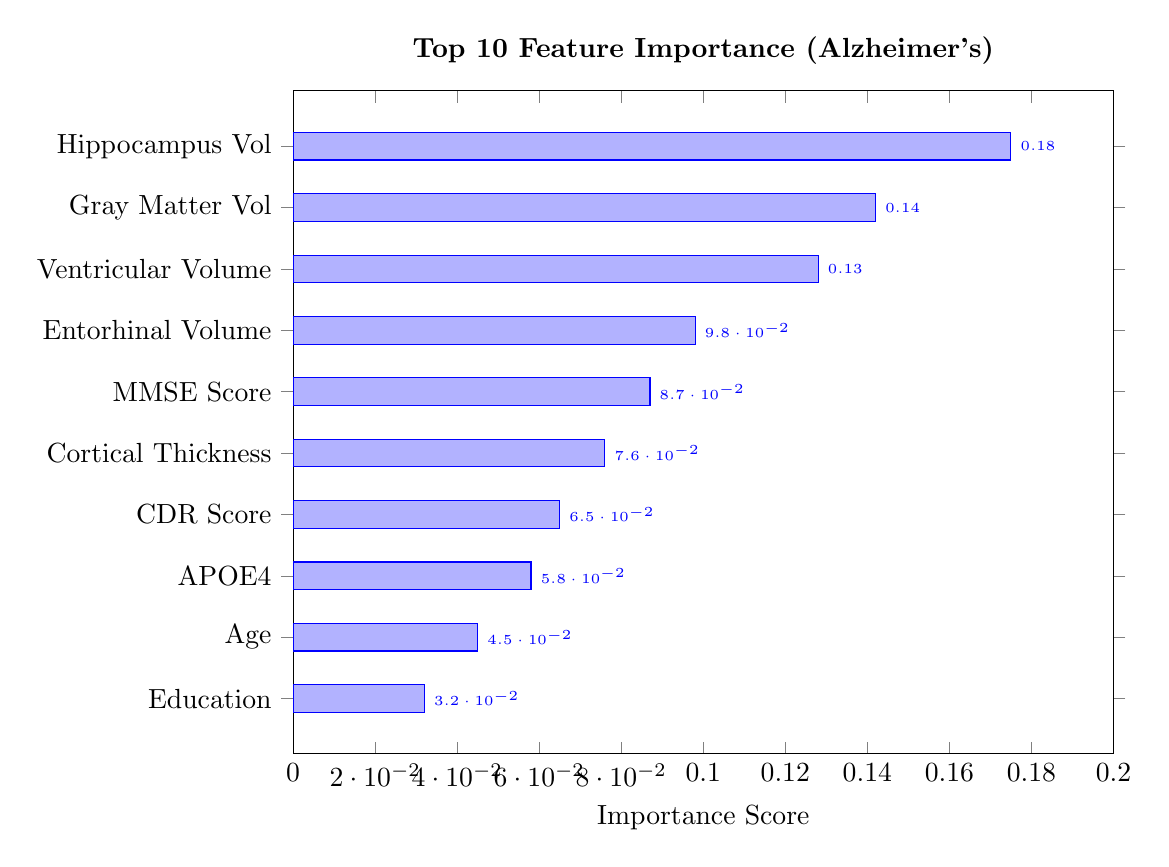
\begin{tikzpicture}
\begin{axis}[
    title={\textbf{Top 10 Feature Importance (Alzheimer's)}},
    xbar,
    bar width=10pt,
    width=12cm,
    height=10cm,
    xlabel={Importance Score},
    symbolic y coords={
        Education,
        Age,
        APOE4,
        CDR Score,
        Cortical Thickness,
        MMSE Score,
        Entorhinal Volume,
        Ventricular Volume,
        Gray Matter Vol,
        Hippocampus Vol
    },
    ytick=data,
    xmin=0,
    xmax=0.2,
    nodes near coords,
    nodes near coords align={horizontal},
    every node near coord/.append style={font=\tiny},
]
\addplot coordinates {
    (0.175,Hippocampus Vol)
    (0.142,Gray Matter Vol)
    (0.128,Ventricular Volume)
    (0.098,Entorhinal Volume)
    (0.087,MMSE Score)
    (0.076,Cortical Thickness)
    (0.065,CDR Score)
    (0.058,APOE4)
    (0.045,Age)
    (0.032,Education)
};
\end{axis}
\end{tikzpicture}

%% ============================================
%% FIGURE 7: Cross-Validation Results
%% ============================================
\begin{tikzpicture}
\begin{axis}[
    title={\textbf{5-Fold Cross-Validation Results}},
    boxplot/draw direction=y,
    ylabel={Accuracy (\%)},
    xtick={1,2,3},
    xticklabels={Alzheimer's, Parkinson's, Schizophrenia},
    ymin=85,
    ymax=100,
    width=12cm,
    height=8cm,
]
% Alzheimer's
\addplot+[boxplot prepared={
    lower whisker=92.1,
    lower quartile=93.2,
    median=94.2,
    upper quartile=95.1,
    upper whisker=96.0
}, fill=red!30] coordinates {};

% Parkinson's
\addplot+[boxplot prepared={
    lower whisker=90.2,
    lower quartile=91.5,
    median=92.8,
    upper quartile=94.0,
    upper whisker=95.5
}, fill=blue!30] coordinates {};

% Schizophrenia
\addplot+[boxplot prepared={
    lower whisker=86.5,
    lower quartile=88.0,
    median=89.5,
    upper quartile=91.0,
    upper whisker=92.5
}, fill=green!30] coordinates {};
\end{axis}
\end{tikzpicture}

%% ============================================
%% FIGURE 8: Deep Learning Architecture
%% ============================================
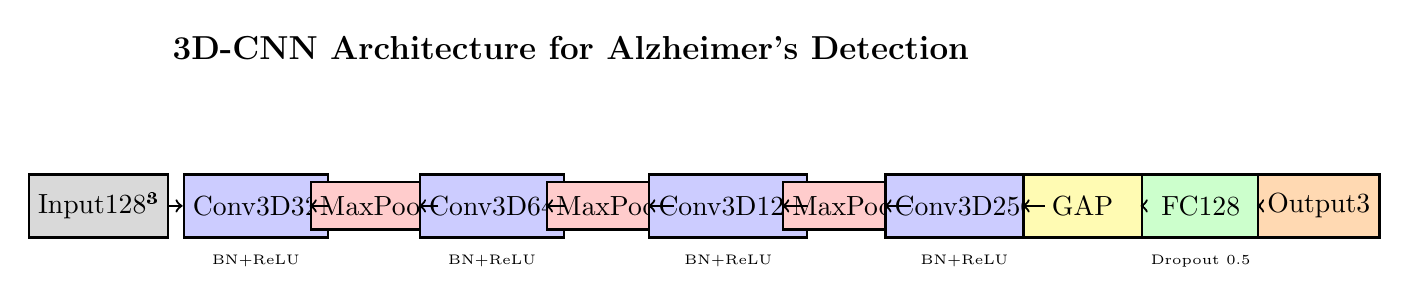
\begin{tikzpicture}[
    node distance=0.8cm,
    conv/.style={rectangle, draw, thick, minimum width=1.5cm, minimum height=0.8cm, fill=blue!20},
    pool/.style={rectangle, draw, thick, minimum width=1.2cm, minimum height=0.6cm, fill=red!20},
    fc/.style={rectangle, draw, thick, minimum width=1.5cm, minimum height=0.8cm, fill=green!20},
    arrow/.style={->, thick}
]

\node[font=\large\bfseries] at (0,3) {3D-CNN Architecture for Alzheimer's Detection};

% Input
\node[conv, fill=gray!30] (input) at (-6,1) {Input\\128³};

% Conv blocks
\node[conv] (conv1) at (-4,1) {Conv3D\\32};
\node[pool] (pool1) at (-2.5,1) {MaxPool};
\node[conv] (conv2) at (-1,1) {Conv3D\\64};
\node[pool] (pool2) at (0.5,1) {MaxPool};
\node[conv] (conv3) at (2,1) {Conv3D\\128};
\node[pool] (pool3) at (3.5,1) {MaxPool};
\node[conv] (conv4) at (5,1) {Conv3D\\256};

% Classifier
\node[fc, fill=yellow!30] (gap) at (6.5,1) {GAP};
\node[fc] (fc1) at (8,1) {FC\\128};
\node[fc, fill=orange!30] (out) at (9.5,1) {Output\\3};

% Arrows
\draw[arrow] (input) -- (conv1);
\draw[arrow] (conv1) -- (pool1);
\draw[arrow] (pool1) -- (conv2);
\draw[arrow] (conv2) -- (pool2);
\draw[arrow] (pool2) -- (conv3);
\draw[arrow] (conv3) -- (pool3);
\draw[arrow] (pool3) -- (conv4);
\draw[arrow] (conv4) -- (gap);
\draw[arrow] (gap) -- (fc1);
\draw[arrow] (fc1) -- (out);

% Annotations
\node[font=\tiny] at (-4,0.3) {BN+ReLU};
\node[font=\tiny] at (-1,0.3) {BN+ReLU};
\node[font=\tiny] at (2,0.3) {BN+ReLU};
\node[font=\tiny] at (5,0.3) {BN+ReLU};
\node[font=\tiny] at (8,0.3) {Dropout 0.5};

\end{tikzpicture}

\end{document}
